%\documentclass[12pt]{article}
\documentclass[BCOR=26.2mm,DIV11,titlepage,a4paper,oneside]{scrbook}
\usepackage{scrhack}
\usepackage[ngerman]{babel}
\usepackage[utf8x]{inputenc}
\usepackage{amsmath}
\usepackage{graphicx}
\usepackage{caption}
\usepackage[colorinlistoftodos]{todonotes}
\usepackage{subcaption}

%fancyheadings funktioniert nicht mehr mit der KOMA Script Klasse scrbook

\usepackage{wrapfig}

\usepackage[authoryear,round]{natbib}

% Mittels [H] können Bilder genau an einer Stelle positioniert werden
\usepackage{float}
\usepackage{hyperref}
% bewirkt das HyperLinks in der PDF nicht umrandet oder farbig sind
\hypersetup{colorlinks=false}

%Paket zur Erzeugung von Anführungszeichen durch \enquote{Text}
\usepackage[ngerman]{babel}
\usepackage[babel, german=quotes]{csquotes}

%Verhindern, dass eine neue Seite für ein einzelnes Wort/Zeile verwendet wird
\clubpenalty = 10000 % schliesst Schusterjungen aus 
\widowpenalty = 10000 % schliesst Hurenkinder aus (keine Beleidigung, sondern wirklich ein Fachbegriff)

\begin{document}

%!TEX root = ../Masterthesis.tex
\begin{titlepage}

\begin{center}
\begin{figure}[!ht]
	\centering
		\includegraphics[width=\textwidth]{images/th_color_bar.png}
\end{figure}
\end{center}
%Deutscher Titel
\begin{flushleft}
\begin{Large}
Masterthesis Medientechnolgie\\
\end{Large}
\vspace{0.5cm}
\begin{LARGE}
\textbf{RHOT-A real-time hand and object tracking system with low cost consumer grade hardware}
\end{LARGE}
\end{flushleft}
\vspace{1.0cm}
\begin{flushleft}
\begin{Large}
vorgelegt von\\ 
\vspace{0.3cm}
\begin{LARGE}
\textbf{Oliver Kalbfleisch} \\
\end{LARGE}
\end{Large}
\end{flushleft}
\vspace{2.0cm}
\begin{flushleft}
\begin{Large}
Erstgutachter: Prof. Dr. Arnulph Fuhrmann(TH Köln) \\[1.0em]
Zweitgutachter: Prof. Dr. Stefan Michael Grünvogel(TH Köln)
\end{Large}
\end{flushleft}
\vspace{1.5cm}
\begin{flushleft}
\begin{large}
Juni \the\year
\end{large}
\end{flushleft}
\begin{figure}[!ht]
\begin{flushright}

\includegraphics[width=0.25\textwidth]{images/TH_bottom_logo.png}
\end{flushright}
\end{figure}
\newpage
\setcounter{page}{1}
\pagenumbering{gobble}
\huge\textbf{Masterarbeit}\\\\
\large
Titel: RHOT Ein echtzeit Hand- und Objektrackingsystem basierend auf kostengünstiger Hardwarekomponenten\\
\textbf{Gutachter}:\\
	Prof. Dr. Arnulph Fuhrmann (TH Köln)\\
	Prof. Dr. Stefan Michael Grünvogel (TH Köln)\\
	\todo{übersetzen}
Zusammenfassung:\\ This paper will evaluate if it is possible to build a hand and object tracking system on low cost consumer grade hardware components. To keep system cost low, a set of Raspberry Pi's with the matching Camera is used for image acquiring an processing. These processing units are linked to a master unit which takes care of stereoscopic depth calculations, the position value processing and the final rendering of a hand and object model in digital space. Several forms of colored marker types are assessed for the prototype application and compared in terms of tracking precision and limiting factors in terms of haptic restrictions for the fingers. The final results show that it is possible to achieve a tracking system solution with the used hardware components that has a suitable tracking update frequency and precision.\\
\textbf{Stichwörter}: Echtzeit,Inverse Kinematik, Hand-tracking, color-tracking,Objekt-tracking, günstig)\\
\textbf{Sperrvermerk}: (optional) Die Einsicht in diese Arbeit ist bis zum TT. Monat JJJJ gesperrt.\\
\textbf{Datum}: TT. Monat JJJJ\\
\newpage
\huge \textbf{Masters Thesis}\\\\
\large
\textbf{Title}: RHOT A real time hand and object tracking system with low cost consumer grade\\
\textbf{Reviewers}:\\
	Prof. Dr. Arnulph Fuhrmann (TH Köln)\\
	Prof. Dr. Stefan Michael Grünvogel (TH Köln)\\
\textbf{Abstract}: \\This paper will evaluate if it is possible to build a hand and object tracking system on low cost consumer grade hardware components. To keep system cost low, a set of Raspberry Pi's with the matching Camera is used for image acquiring an processing. These processing units are linked to a master unit which takes care of stereoscopic depth calculations, the position value processing and the final rendering of a hand and object model in digital space. Several forms of colored marker types are assessed for the prototype application and compared in terms of tracking precision and limiting factors in terms of haptic restrictions for the fingers. The final results show that it is possible to achieve a tracking system solution with the used hardware components that has a suitable tracking update frequency and precision.\\
\textbf{Keywords}: Hand-tracking, Object-tracking, inverse kineamtics, low-cost, realtime \\
\textbf{Date}: 29 June 2018\\

\end{titlepage}


\tableofcontents
\setcounter{page}{1}
\newpage

\chapter*{Kurzfassung}
Hier folgt die Kurzfassung.

\newpage
\chapter*{Abstract}
Hier folgt die Kurzfassung auf Englisch.

\newpage
%!TEX root = ../main.tex
\pagenumbering{arabic}
\chapter{Einleitung}
The standard interface between human and computer has for long years been mouse and keyboard. But with the advance of technology, new interfaceing methods were developed in the last few years.\\
Touch technology for interfacing with mobile devices and desktop computers has become a reliable technology and has been integrated into our everyday lives.
Advances in  capabilites of CPU as well as GPU hardware has build a foundation for the use of advanced AR and VR Technology. 3D and Stereoscopic rendering can now be accomplished even by mobile hardware (with some limitations) without the need of specifci hardware. For an intensly immersive experience VR Googles are used to explore digitally created worlds.\\
But with this level of immerivenes, a touch device or even a mouse and keyboard setup is rather hindering the user experience. First attempts of solving this problem came with the introduction of tracked controllers for the interaction with the digital world, but these can also only supply a fration of the capabilities of our natural interaction devices, namely the human hands.\\This thesis aims to display a method of combining the tracking of a physical object and the human hand(s) and merging this data into the digital space. The resulting experience for the user should be as natural as possible. Therefore  different systems for tracking of objects and bodyparts as well as the display of these in digital space will be presented and assessed. The results from the assessment wil be incorporated into a system prototype for testing with real users.
\newpage
%!TEX root = ../main.tex
\chapter{Kapitel 1}

\section{Section}
sadfsdf
\section{Section}
Beispiel für eine Tabelle:
\begin{table}[ht]
	\centering
	\caption[Kurztitel Tabelle]{Hier steht die lange \underline{\textbf{ÜBER-}}schrift für die Tabelle}

		\vspace{1.0em}
		\begin{tabular}{|l|r|}
\hline
Text & 12\% \\
\hline
Text & 34\% \\
\hline
Text & 56\% \\
\hline
Text & 78\% \\
\hline
Text & 90\% \\
\hline
		\end{tabular}
	\label{tab:tabelle}
\end{table}


\noindent{}Dies ist lediglich ein Beispiel. Je nach beabsichtigter Aussage, können Tabellen ganz unterschiedlich aussehen. Allerdings haben Tabellen eine \emph{Über}schrift, während es sich bei Abbildungen um \emph{Unter}schriften handelt.

\section{Section}

\section{Section}
siehe Tabelle \ref{tab:tabelle}

\subsection{Subsection}

\subsection{Subsection}
\newpage
%!TEX root = ../MAsterthesis.tex


\chapter{Description of hand in digital space}
Tracking of the human hand has always been a challenging Problem. In comaprison to other larger bodyparts like the Arm or the head, the human hand itself contains a large variety of smaller parts, namely bones and muscles. These components have to be taken into acount when trying to replicate the natural motion of the hand in digital space.\\
\section{Physiological structure of the human hand}
\citep{LEE.1995} describes the human hand as "an articulated structure with about 30 degrees of freedom [which] changes shape in various ways by its joint movemnents."
\begin{figure}[H]
	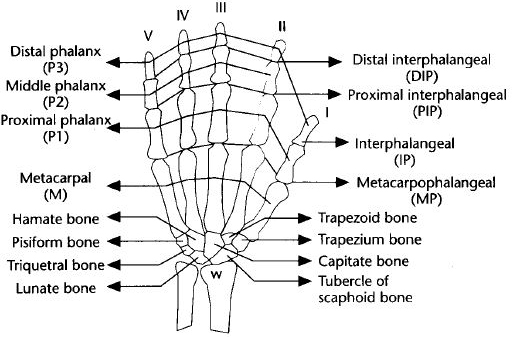
\includegraphics[scale=0.8]{images/hand.jpg}
	\label{Handstructure} 
	\caption{Bone structure of the human left hand (\cite{LEE.1995})}
\end{figure}
All of the hand components are connected to at least one neighboring component via a joint. Teh joints affect the position of the connected components. To describe the movement of the hand components, we can use the roation angles of the joints to correlate to a specific position.\\
To do so, we define a local coordinate system for each of the exiting hand joints. By doing so, we achieve a sequence of rotaions in the local coordinate systems of the joints. Such a sequence can then be used to describe a specific movement and/or position of a component.
Not all of the joints in the human hand have equal degrees of freedom. Their functionality can be classified in the amount of DOFs (Degrees of freedom)\cite{KOREIN.1985}
\begin{itemize}
\item 1 DOF \\
	- A joint movement that can perfom a \textbf{flexion} or \textbf{twist} in one direction
\item 2 DOF \\
	- A joint movement that can perform \textbf{flexion} in more than one direction (\textbf{directive})
\item 3 DOF\\
	- A joint movement that permits simultaneous \textbf{directive} and \textbf{twist} movements.(\textbf{spherical})
\end{itemize}
\begin{figure}[H]
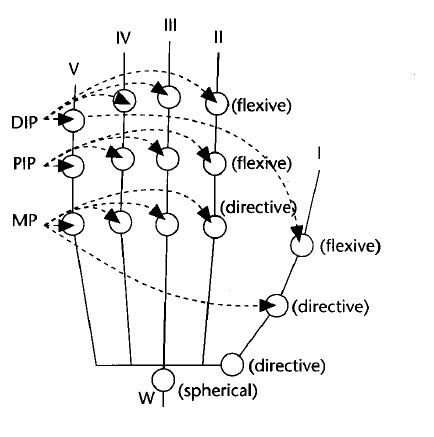
\includegraphics[scale=0.8]{images/Hand_DOFs.JPG} 
\caption{Representation of the DOFs of the human hand}
\label{dof_image} 
\end{figure}
When looking at the DOFs diplayed in Figure \ref{dof_image}, each finger (II-V) sums up to 4 DOFs and the thumb to 5 DOFs. Also considering 6 DOFs for the rotation and position of the whole and itsself, the result gets us to 27 DOFs  for the human hand.
\subsection{Constraints in Hand Motion}
A full usage of all the declared DOFs would lead to al large amount of possible combination. Since the hand is not only made up of bones but also Muscles and the skin, we can impose some constraints( \cite{Badler.1987}) to the movement of the joints. Ling, Wu and Huang(\cite{LIN.2000}) propsed following classification for the constrainsts:
\newpage
\begin{itemize}
\item \textbf{Type I constraints}\\
	-A constraint that limits the range of finger motions based on hand anatomy
	\item \textbf{Type II constraints}\\
	- A constraint that the position of the joints during finger movement
	\item \textbf{Type III constraints\\}
	-A constraint that limits position based on natural hand motions
\end{itemize} 
The \textbf{Type I} and \textbf{Type II} constarints rely on the physiological and mechanical properties of the humand.\textbf{Type III} constraints are results of common and natural
movements and can be differing form person to person. As these movements are to some degree simular for everyone, a broad grouping can be applied. The curling of the fingers at the sane time when forming a fist is way more natural than curling each finger by itsself. Here the motion of the hand is quite simular between different persons, but the constraints cannot be described in a mathematical form. \\
 A \textbf{Type I} constraint example would be that the position of the fingertip is kimited by the length of the other finger segments and therby can only reach as far as the combined length.\\An example for \textbf{Type II} constraints would be that, for your fingertip to touch your hand palm, all joints in the finger have to be bend to achieve this position.
The following inequalities can be used to describe these constraints:\\
\textbf{Type I:}
\begin{equation}
\begin{split}
0°&\leq \Theta _{MP\_flex} \leq 90°\\
0°&\leq \Theta _{PIP\_flex} \leq 110°\\
0°&\leq \Theta _{DIP\_flex} \leq 90°\\
-15°&\leq \Theta _{MP\_abduct/adduct} \leq 15°
\end{split}
\end{equation}
A further constraint that is specific to the middle finger is, that this fingers MP normally does not abduct and adduct much. Therefore we can infer an approximation and thereby remove 1DOF from the model:
\begin{equation}
\Theta _{MP\_abduct/adduct}=0°
\end{equation}
The same behavior can be seen in the combination of hand parts labeled W(the connection point between hand and lower arm). This approximation allso eliminates one DOF on the connected thumb:
\begin{equation}
\Theta _{W\_abduct/adduct}=0°
\end{equation}
Since the DIP,PIP and MP jonts of our index, middle, ring, and little fingers only have 1DOF for flexion, we can further asume that their motion is limited to movement in one plane. \\
\textbf{Type II:}\\
The \textbf{Type II} constraints can be split into interfinger and intrafinger constraints. Regarding intrafinger constraints between the joints of the same finger, human hand anatomy implies that to bend the DIP joints  on  either the index, middle, ring or little fingers,the corresponding PIP joints of thath finger must also be bent. The approximation for this relation\cite{Rijpkema.1991} can be described as :

\begin{equation}
\Theta _{DIP} =\frac{2}{3}\Theta _{PIP}
\end{equation}
Interfinger constraints can be imposed between joints of adjacent fingers. Interfinger constraints describe that the bending of an MP joint in the index finger forces the MP joint in the middle finger to bend as well.\\
 When combinig the constraints described in the above equations, the starting number 21 DOF's of the human hand can be reduced to 15. Inequalities for these cases, obtained through empiric studies, can be found in \citep{LEE.1995}.\\
\section{Kinematics}
 The preceeding sections gave an overview of how we can describe a model of the human hand and introduced some limiting constraints. With the model and the constraints, we can now start to build a kinematic system for the animation of the model.\\
Kinematic systems contain so called \textit{kinematic chains}, which consist of a \textit{starting point}or \textit{root}, kinematic elements like \textit{joints}, \textit{links} and an \textit{endpoint}, also called \textit{end effector}. Applied to the human hand, the whole hand model represents the kinematic system. This system contains several \textit{kinematic chains}, namely the fingers of the hand with the fingertips beeing the \textit{end effectors} of each of these chains.\\
As we begin to move our hands, the states of the kinemtic chains begin to change. Joint angles and end effector positions are modified until the end position is reached. To represent the new position and agnle dataset of our physical hand with our kinematic system, two major paths for achieving a solution can be taken.
 \subsection{Forward Kinematics}Forward
 \label{Forward Kinematics}  Kinmatics (FK) uses the knowledge of the new angles and positions after the application of known transformations to the kinematic chain. The data of the \textit{joints} and \textit{links} between the \textit{root} and the \textit{end effector} is then used to solve the problem of finding the \textit{end effector's} position.\\
We can denote the exisiting end effectors relative postion to an origin as $ s_{1},...,s_{k}$. The $s_{i}$ positon is the result of th combination of all the joint angles in the corresponding kinemtaic chain. Respectively, we define the target positon of the end effectors as $t_{1},...,t_{i}$, with $t_{i}$ beeing the target positiojn for the end effector $s_{i}$. The required positional change for the end effector can now be described as $e_{i}=t_{i}-s_{i}$. In systems with more than one end effector, like our hand system, the components can be written as vectors.
\begin{equation}
\label{fk components}
\begin{split}
\vec{\textbf{s}}&=(\textbf{s}_{1},...,\textbf{s}_{n})^{T}\\
\vec{\textbf{t}}&=(\textbf{t}_{1},...,\textbf{t}_{n})^{T}\\
\vec{\textbf{e}}&= \vec{\textbf{t}}-\vec{\textbf{s}}
\end{split}
\end{equation}
As the vector components of $\vec{\textbf{s}}$ are reults of the chain joint angles $\theta_{1},...,\theta_{n}$ and therefore are effected by them, we define 
\begin{equation}
\label{forward kinematic solution}
\begin{split}
\vec{\textbf{s}_{i}}&=f_{i}(\pmb{\theta})\\
\vec{\textbf{s}}&=f(\pmb{\theta})\\
\end{split}
\end{equation}
with $\pmb{\theta}$ beeing the column vector $\pmb{\theta}=(\theta_{1},...,\theta_{n})^{T}$.The second vector equation displayed in (\ref{forward kinematic solution}) is also callled the \textit{Forward Kinematics}(FK) solution.\\
\\The advantage of an FK solution is that there is always an unique solution to the problem. In consequence, this approach is commonly used in the field of robotics, where the information on the chain elements is easily available.\\
The tracking of the human hand and all if its chain components is rather complicated.Therefore a solution which takes a known position of the \textit{end effektor} and calculates the parameters for the rest of the cain would be more desireable.\\

 \subsection{Inverse Kinematics}
 \label{inverse kinematics}
\begin{quote}Inverse Kinematics (IK) is a method for computing the posture via estimating each individual degree of freedom in order to satisfy a given task~\cite[S.~14]{AndreasAristidouandJoanLasenby.}\end{quote}
The concept of \textit{Inverse Kinematics}  (IK) already describes it's principle in it's name. It takes the reversed approach in comparison to the FK principle in chapter \ref{Forward Kinematics}. Instead of knowing the states of the chain elements and calculating the resulting position of the \textit{end effector}, we take the position of the \textit{end effector} and try to retrieve the possible states of the other chain elements. 
\begin{equation}
\label{ik problem formula}
\pmb{\theta}=f^{-1}(\vec{\textbf{s}_{d}})
\end{equation}
The result of this equation is the vector $\pmb{\theta}$ for which the values of $\vec{\textbf{s}}$ coincide to the desired configuration $\vec{\textbf{s}_{d}}$. In the case of an optimal result, this configuration would have the same position values as the target positions.\\ The main problem with this method occurs in the calulaton of the $f^{-1}$ function, due to it beeing a highly non linear operator which is not easily invertible. Some of the approaches that are used to counter this problem will be displayed later on in this chapter.\\
\\In contrary to having a unique solution with the FK approach, the IK approach can end at the point of not finding a suitable solution. Figure \ref{IkSolutions} diplays three possible outcomes for the IK approach.
\begin{figure}[H]
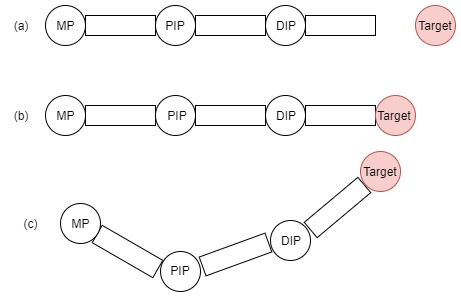
\includegraphics[scale=0.6]{images/Ik_figure.jpg}
\caption{Possible solution for an IK problem of a human finger:\\(a)The given target position of the end effector can not be reached. (b) The given target can only be reached by one solution.(c) The target position can be reached with multiple different solutions.}
\label{IkSolutions}
\end{figure}
\subsubsection{Nonlinear Programming}
\subsubsection{Jacobian Inverse}
One common approach to solve the IK problem is the utilization of a Jacobian Matrix and an iterative calulaton process. This matrix contains the partial derivates of the chain systems relative to the end effector \textbf{s}. When using the Jacobian, a linear approximation  of the IK problem will be applied for solving. The approximation's components model the end effector's realtive movement to changes in transitions of the systems link translations and joint angles. Therefore, the resulting function is dependant on the joint angles $\pmb{\theta}$ values and can be defined as
\begin{equation}
\label{Jacobian definition}
J(\pmb{\theta})_{ij}=\left(\frac{\partial\textbf{s}_{i}}{\partial\theta_{j}}\right)_{ij}
\end{equation}
with \textit{i}=1,...,k and \textit{j}= 1,...,n.
Further readings on methods for the calculation of Jacobian matrices can be found in \cite{Orin.1984}. Based on definition (\ref{Jacobian definition}), an entry for the j-th rotational joint would be calculated as follows:
\begin{equation}
\label{Jacobian entry calc}
\frac{\partial \textbf{s}_{i}}{\partial \theta_{j}}= \textbf{v}_{j}\times(\textbf{s}_{i}-\textbf{p}_{j})
\end{equation}
where $\textbf{p}_{j}$ is the position of the joint, and $\textbf{v}_{j}$ is the unit vector pointing along the current axis of rotation for the joint.
Taking the derivate of definition (\ref{forward kinematic solution}) with respect to time gives the basicequation for forward kinematics that describes the velocities of the end effectors:
\begin{equation}
\label{fk derivate}
\dot{\vec{\pmb{s}}}=\pmb{J}\pmb{(\theta)}\dot{\pmb{\theta}}
\end{equation}
\\ Now having all the values for the anlges, the \textit{end effector} position and the target positions, we can compute the resulting Jacobian matrix.
Thereafter we seek an update value $\Delta\pmb{\theta}$ for incementing the current joint values:
\begin{equation}
\label{theta calc}
\pmb{\theta}_{new}=\pmb{\theta}_{curr}+\Delta\pmb{\theta}
\end{equation}
The idea here is that the  chosen value for $\Delta\pmb{\theta}$ should lead to the resulting $\Delta\pmb{\vec{s}}$ beeing approximately equal to $\vec{\textbf{e}}$ from (\ref{fk components}). The $\vec{\textbf{e}}$ can be approximated by:
\begin{equation}
\label{delta s approx}
\Delta\pmb{\vec{s}}\approx \pmb{J(\theta_{curr})}\Delta\pmb{\theta}
\end{equation}
Using this approximation  we can reformulate the FK problem as $\pmb{}\vec{\pmb{e}}=J\Delta\pmb{\theta}$ and therefore our inverse kinematics problem form \ref{ik problem formula} can be expressed as $ \Delta\pmb{\theta}=J^{-1}\vec{\pmb{e}}$. \\The problem we run into with this solution is the construction of the inverse Jacobian matrix. The Jacobian J may not be square or invertible. In the case of it beeing invertible , the result may only work inferiorly because of it beeing nearly singular. Beeing singular means that no change in joint angle values may achieve the desired end effector position as an outcome.
\subsubsection{Jacobian Transpose}
One approach to calculating the value of $\Delta\pmb{\theta}$ without having to calcualte the inverse of \textbf{J} is done by relpacing the inverse with the transpose of \textbf{J}.
\begin{equation}
\label{delta s approx}
\Delta\pmb{\theta}=\alpha \pmb{J}^{T}\vec{\pmb{e}}
\end{equation}
Of course the transpose and the inverse of \textbf{J} are not the same thing. When using the theorems displayed in \cite{.1984b,Wolovich.1984} we can show that: 
\begin{equation}
\label{transpose show}
\langle JJ^{T}\vec{\pmb{e}},\vec{\pmb{e}}\rangle=\langle J^{T}\vec{\pmb{e}},J^{T}\vec{\pmb{e}}\rangle=\|J^{T}\vec{\pmb{e}}\|\geq 0
\end{equation}
Under a sufficiently small $\alpha>0$ the updated angles from \ref{theta calc} will change the end efector positions by approximately $\alpha JJ^{T}\vec{\pmb{e}}$. They also state that 
the value of $\alpha$ can be calculated by minimising the new value of the error vector $\vec{\pmb{e}}$ after each update.
\begin{equation}
\label{transpose show}
\alpha=\frac{\langle\vec{\pmb{e}},JJ^{T}\vec{\pmb{e}}\rangle}{\langle JJ^{T}\vec{\pmb{e}},JJ^{T}\vec{\pmb{e}}\rangle}
\end{equation}
\subsubsection{Jacobian Pseudo Inverse}
Instead of calculating the normal inverse of the Jacoboian, which can lead to the problems described before, we can use the so called \textit{pseudo-inverse}\cite{Dahmen.2008} for the calculation. The \textit{pseudoinverse} is defined for all matrices J, even ones
which are not square or not of full row rank.
\begin{equation}
\label{pseudo inv def}
\Delta\pmb{\theta}=J^{\dagger}\vec{\pmb{e}}
\end{equation}
\\The \textit{pseudoinverse} represents the best possible solution for $ J\Delta\pmb{\theta}=\vec{\pmb{e}}$ in respect to least squares. It has the favourable properties thath if the $\vec{\pmb{e}}$ Vector lies within the range of the \textbf{J}





First, suppose ~e is in the range (i.e., the
column span) of J . In this case, J∆θ = ~e; furthermore, ∆θ is the unique
vector of smallest magnitude satisfying J∆θ = ~e. Second, suppose that ~e
is not in the range of J . In this case, J∆θ = ~e is impossible. However,
∆θ has the property that it minimizes the magnitude of the difference
J∆θ − ~e. Furthermore, ∆θ is the unique vector of smallest magnitude
which minimizes ||J∆θ −~e||, or equivalently, which minimizes ||J∆θ −~e||2 .


\subsection{FABRIK Algorithm}

 A more recent approach in the kinematics field is the \textbf{FABRIK} algorithm proposed by Aristidou
 and Lasenby\cite{Aristidou.2011}.As shown in section \ref{inverse kinematics}, these approaches all depend on computational intensive matrix operation like calculating an inverse and may have problems with matrix singularity.\\
\begin{wrapfigure}{r}{0.61\textwidth}
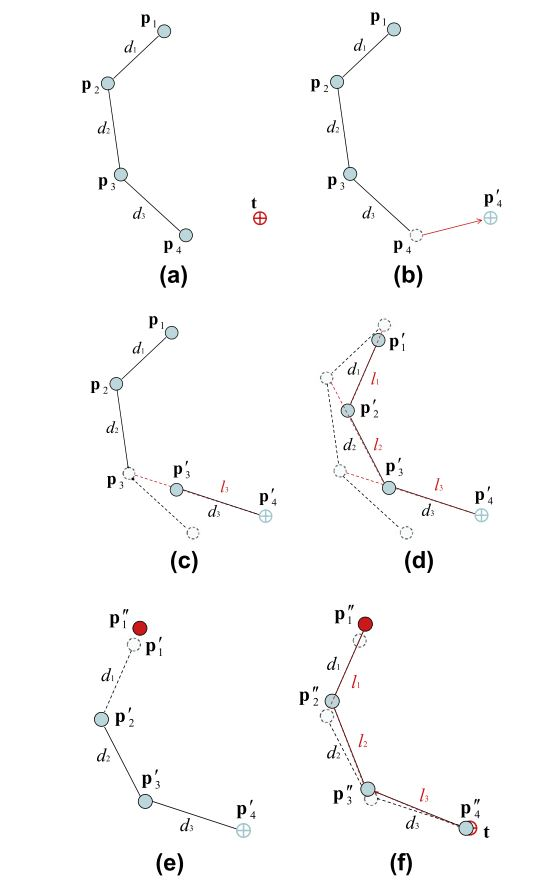
\includegraphics[scale=0.61]{images/FabrikIteration.jpg}
\caption{Forward and backward calculation steps for one iteration of the \textbf{FABRIK}algorithm.(a) initial position of the system.(b)End effector is moved to target position.(c) Deterimne position of next joint on constructed line.(d)repeat until root is reached. (e)move root joint to initial position. (f) repeat calculation in reverse direction \cite{Aristidou.2011} }
\label{Fabrik_Iteration}
\end{wrapfigure}
The \textbf{FABRIK} algorithm does not depend on these matrix operations as is solves for the position of a point on a line to retrieve the new joint positions. This is done in an forward and also inverse solving approach, itterating these steps until the calculated position converges towards the target position from the tracking data.\\
Figure \ref{Fabrik_Iteration} illustrates the steps that are contained in one iteration step.
The chain joints are denoted as $\textbf{p}_{\textit{i}}$ with the distance $\textbf{d}_{i}$ being $|\textbf{p}_{\textit{i+1}}-\textbf{p}_{\textit{i}}|$. The target point for the end effector is denoted as \textbf{t}. Step \textbf{(a)} displays the starting pont of the iteration. The joint positions are taken from either a previous iteration or from an initial calibration. \\
But before calculations can begin, the algorithm has to check whether the intended target point \textbf{t} is reachable for the end effector. This is done by measuring the distance between the root of the kinamtic chain and the target point \textbf{t}. This value is then compared with the sum of the distances $\textbf{d}_{i}$.
\begin{equation}
 dist_{t,d_{1}}< \sum_{k=1}^{i}{d_{i}}
\end{equation}\\The inverse calculation step is the first step, which is diplayed in \textbf{(b)} and \textbf{(c)}.The calculation is started at the end effector, moving to the root of the chain. 
If the summed distance is greater, then the \textbf{t} is within the reach of the system and the calculation can continue, otherwise the calculation has to be aborted and the error has to be manged otherwise.
Assuming this requirement to be met, we can now begin with the first calculation. Therefore we assume that the new position $\textbf{p}_{n}^{'}$ with n=4,...,1 is equal to \textbf{t}.
\begin{equation}
 \textbf{p}_{n}^{'}=\textbf{t}
\end{equation}\\
From this new point, we can construct a line that goes through $\textbf{p}_{n}^{'}$ and $\textbf{p}_{n-1}$.
\begin{equation}
\begin{split}
A&=\textbf{p}_{n}^{'}\\
B&=\textbf{p}_{n-1}\\
\textbf{l}_{n-1}&=\overline{AB}\\
\end{split}
\end{equation}
The resultng position of the new $\textbf{p}_{n-1}^{'}$ point is located in this line with the distance of $\textbf{d}_{n-1}$ from $\textbf{p}_{n}^{'}$ (see \textbf{(c)}).
\begin{equation}
\textbf{p}_{n-1}^{'}= \textbf{p}_{n}^{'}+ \left(\frac{\overline{AB}}{|\overline{AB}|}\cdot\textbf{d}_{n-1}\right)
\end{equation}
Consecutively, this is done with the remaining joints until the root joint is reached(see \textbf{(d)}).
This finishes the first halv of the iteration step.With the calculated positions, we now perform a forard calculation, starting from the root until we reach the end effector. Since the root of the system normally does not move from it's initial position, we have to reset the root jont to this value before starting to calculate the new positions of the subsequent joints(see\textbf{(e)}).

Analogous to the procedure in the inverse step, we construct the lines between the points and determine the new positon values of the joints. The end result of this step is shown in \textbf{(f)}. At this point, we can decide if the result position of the end effector is appropriate in comparison to the value of \textbf{t}. A simple threshold value for this case could be the position difference between these two points.

\section{Digital hand models}
\newpage
\chapter{Resume}

Future work:\\
-improve depth tracking value preciion through a more elaborate calibration seesion where the depth correcton algorith is further optimized
\\
-improve image reading source code to accept hgher framerates. The hardware capacbilities provide image reading frequences of up to 90fps, current bottleneck is the c++ implementaion which only provides 30 fps max.
\\
-When utilizng higher framerates, the multiproceesng approach will be viable to gain performance. Optimizaton work on the implementaion can be done.\\
-Image manipulaton on the cpu is rather costly, even at small image sizes. The raspberry Pi has a "small" gpu unit onboard, whch is in dle state when the device is run in headless mode. The gpu could then be utilzed to do heavy weight image calculation such as stereo rectification.\\
-Optimization pont would also be creating a mor optimized verson of the color thresholding algorithm where the threshoding for all of the thracking colors is done in one run on the current frame. It is also to be evaluated if ths problem falls can be expressed as a SIMD functon and would benefit from the processng on the gpu.
\\
The current prototype is still missing an graphcal user interface on the display side. Further communication of states on the slave Pi's to the master unit would also be beneficial.
\\
The habd data that is used for prototyping is still hardcoded and only manually configurable. A calibration procedure for the system as well as a suitable data format for representing and translating these values for the IK algortihm s still to be done.
\\
-Shrnk tubing showed to be a utilzable material for the usecase. Downsinde of the material is that the colors used are the largest spectrum of colors available on the market and geting outer colors is relatively hard. Other materal shuold be evaluated.



\newpage
%Erzeugt ein Abbildungsverzeichnis
\pagenumbering{roman}
	\listoffigures
	%Fügt die Zeile "`Abbildungsverzeichnis"' als Chapter ins Inhaltsverzeichnis ein
	\addcontentsline{toc}{chapter}{Abbildungsverzeichnis}
\newpage
	
	%Erzeugt ein Tabellenverzeichnis
	\listoftables
	%Fügt die Zeile "`Tabellenverzeichnis"' als Chapter ins Inhaltsverzeichnis ein
	\addcontentsline{toc}{chapter}{Tabellenverzeichnis}
\newpage

% To change the title from References to Bibliography:
\renewcommand\refname{Literaturverzeichnis}

%Paket für ein deutsches Literaturverzeichnis

\bibliography{literature} % refers to literatur.bib

	%Fügt die Zeile "`Literaturverzeichnis"' als Chapter ins Inhaltsverzeichnis ein
	\addcontentsline{toc}{chapter}{Literaturverzeichnis}
\newpage

%!TEX root = ../Masterthesis.tex
\chapter*{Eidesstattliche Erklärung}
%\addcontentsline{toc}{chapter}{Eidesstattliche Erklärung}

Ich versichere, die von mir vorgelegte Arbeit selbständig verfasst zu haben.\\ 
Alle Stellen, die wörtlich oder sinngemäß aus veröffentlichten oder nicht veröffentlichten Arbeiten anderer entnommen sind, habe ich als entnommen kenntlich gemacht. Sämtliche Quellen und Hilfsmittel, die ich für die Arbeit benutzt habe, sind angegeben.\\ 
Die Arbeit hat mit gleichem Inhalt bzw. in wesentlichen Teilen noch keiner anderen Prüfungsbehörde vorgelegen.
\vspace{1.5cm}
\\
Köln, xx. August 2016
\vspace{3cm}
\\
Oliver Kalbfleisch


% chapter eidesstattliche_erklärung (end)

\end{document}